\documentclass[conference]{IEEEtran}
\IEEEoverridecommandlockouts
% The preceding line is only needed to identify funding in the first footnote. If that is unneeded, please comment it out.
\usepackage{cite}
\usepackage{amsmath,amssymb,amsfonts}
\usepackage{algorithmic}
\usepackage{algorithm}
\usepackage{graphicx}
\usepackage{textcomp}
\usepackage{xcolor}
\usepackage{booktabs}
\usepackage{multirow}
\usepackage{tabularx}
\usepackage{tikz}
\usetikzlibrary{arrows,shapes,positioning}

\def\BibTeX{{\rm B\kern-.05em{\sc i\kern-.025em b}\kern-.08em
    T\kern-.1667em\lower.7ex\hbox{E}\kern-.125emX}}

\begin{document}

\title{Adaptive and Resource-Efficient Network Intrusion Detection for Previously Unseen Attacks in IoT Networks}

\author{\IEEEauthorblockN{Chitchula Sai Bhuvan}
\IEEEauthorblockA{\textit{Department of Computer Science and Engineering} \\
\textit{Amrita School of Computing} \\
\textit{Amrita Vishwa Vidyapeetham}\\
Coimbatore, India \\
cb.sc.p2cse25007@cb.students.amrita.edu}
\and
\IEEEauthorblockN{Dr. Panduranga Ravi Teja}
\IEEEauthorblockA{\textit{Department of Computer Science and Engineering} \\
\textit{Amrita School of Computing} \\
\textit{Amrita Vishwa Vidyapeetham}\\
Coimbatore, India \\
p\_raviteja@cb.amrita.edu}
}

\maketitle

% =========================================================================
% 1. ABSTRACT & INDEX TERMS
% =========================================================================
\begin{abstract}
Machine learning based Network Intrusion Detection Systems (NIDS) deployed on edge Internet of Things (IoT) gateways achieve remarkable classification accuracy under static, closed-world benchmarks. However, they fail catastrophically when deployed in adversarial zero-day environments, yielding zero detection recall on previously unobserved attack vectors. Updating edge models on confirmed novel threats introduces an acute operational trilemma: periodic full retraining on historical packet archives causes flash memory exhaustion and prohibitive execution latency; incremental updates trigger catastrophic forgetting of earlier threat signatures; and massive historical archives severely dilute compact zero-day threats during decision tree splitting. 

This paper presents an autonomous, resource-efficient continual intrusion detection framework engineered specifically for resource-constrained edge IoT gateways following a rigorous IMRaD methodology. The architecture couples an unsupervised Isolation Forest novelty screener—which provides an operational out-of-distribution alert trigger without requiring labels—with an on-demand supervised continual adaptation engine powered by a deterministic, volume-aware \emph{Dynamic Replay Buffer}. Rather than relying on arbitrary static buffers, our allocation rule mathematically bounds the volumetric imbalance ratio $\rho$ by dynamically proportioning historical exemplar retention to match incoming novel attack volumes within hardware-enforced memory ceilings ($<1$\,MB). We conduct extensive empirical evaluations on the benchmark TON\_IoT corpus ($183{,}592$ deduplicated network flows across $41$ attributes) across four diverse threat families under a strict leave-one-attack-out protocol. The empirical findings reveal that: (1) closed-world baselines yield an exact 0.0000 F1-score on held-out attacks, misrouting up to $29.26\%$ of malicious flows directly into benign traffic; (2) for low-volume stealth attacks (MITM), class-balanced replay neutralizes Gini impurity dilution, elevating novel-attack F1 from 0.6483 (full retraining) to 0.9773 while reducing exemplar storage by 99.30\% and accelerating training by $11.6\times$; (3) for high-volume volumetric attacks (Ransomware, XSS, Backdoor), our volume-aware Dynamic Replay suppresses maximum catastrophic forgetting by 20.0\%--35.9\% relative to static replay while preserving $>96.7\%$ memory savings; and (4) adaptation updates execute on-device in under 0.085\,seconds. Finally, we establish the framework's ecological and operational viability within the United Nations Sustainable Development Goals (SDG 9, 11, and 12), providing a robust Green AI blueprint for resilient edge computing.
\end{abstract}

\begin{IEEEkeywords}
IoT Security, Network Intrusion Detection, Continual Learning, Catastrophic Forgetting, Dynamic Replay Buffer, Zero-Day Attacks, Decision Tree Induction, Green AI.
\end{IEEEkeywords}

% =========================================================================
% 2. I. INTRODUCTION
% =========================================================================
\section{Introduction}
\label{sec:introduction}

The Internet of Things (IoT) has emerged as the critical nervous system of modern socio-technical infrastructure, interconnecting billions of sensors, industrial programmable logic controllers (PLCs), smart grid gateways, and autonomous cyber-physical systems~\cite{alshammari2020toniot}. Situated at the hostile interface between local operational technology (OT) subnets and external wide-area networks, edge gateways collect, aggregate, and transmit mission-critical telemetry. However, edge IoT hardware is engineered under stringent physical, thermal, and economic constraints. Typical edge appliances operate with minimal volatile memory (RAM), constrained non-volatile flash storage, and low-frequency microprocessors. Consequently, conventional host-based endpoint defense suites—such as deep packet inspection (DPI) engines, heavy cryptographic tunnels, and monolithic signature-based antivirus agents—are computationally and physically infeasible. This structural constraint leaves IoT aggregation gateways vulnerable to an expanding spectrum of cyber threats, ranging from Mirai-style distributed denial-of-service (DDoS) botnets to polymorphic ransomware, firmware backdoors, and stealthy Man-in-the-Middle (MITM) manipulations.

Network Intrusion Detection Systems (NIDS) deployed directly on edge IoT gateways provide the primary defensive perimeter. While supervised machine learning models—particularly decision tree ensembles such as Random Forests~\cite{breiman2001random}—achieve near-perfect classification accuracy ($>97\%$) on static benchmarks, their operational integrity breaks down completely under the \emph{Closed-World Assumption}:
\begin{equation}
\mathcal{P}_{\text{test}}(\mathbf{x}, y) = \mathcal{P}_{\text{train}}(\mathbf{x}, y), \quad y \in \mathcal{C}_{\text{known}} = \{1, 2, \dots, K\}.
\end{equation}
Under this foundational assumption, classifiers assume that all future network flows belong strictly to the taxonomy encountered during offline training. When an adversary deploys a zero-day exploit, a polymorphic evasion, or an out-of-distribution attack vector $\mathbf{x}^* \sim \mathcal{P}_{K+1}$, the classifier is mathematically forced to project $\mathbf{x}^*$ onto the historical label space $\mathcal{C}_{\text{known}}$. This results in silent intrusion evasion, catastrophic false negatives, and severe collateral misclassification across familiar traffic classes.

\subsection{The Plasticity--Stability Dilemma on Edge Gateways}
When network security analysts or automated security orchestration platforms identify an ongoing zero-day intrusion, the edge gateway must assimilate the novel threat. However, on-device model updating encounters the classical \emph{Plasticity--Stability Dilemma}~\cite{de2021continual}:
\begin{itemize}
    \item \textbf{Plasticity:} The agility of the model to establish tight decision boundaries for the newly emerging attack class ($K+1$).
    \item \textbf{Stability:} The capability of the model to retain previously learned decision boundaries, preserving detection fidelity on the original $K$ classes.
\end{itemize}

If an edge detector is fine-tuned or retrained exclusively on the confirmed novel attack batch, it suffers \emph{Catastrophic Forgetting}~\cite{kirkpatrick2017overcoming}: the tree induction algorithm recursively overwrites historical feature splits, eradicating legacy knowledge and rendering the gateway defenseless against familiar exploits.

Conversely, the conventional countermeasure—\emph{Full Historical Retraining} (joint retraining from scratch)—requires permanently storing all historical network telemetry on the edge device. This approach fails on edge hardware due to three critical bottlenecks:
\begin{enumerate}
    \item \textbf{Flash Memory Exhaustion:} Edge gateways lack the non-volatile storage required to maintain hundreds of megabytes of raw historical packet archives.
    \item \textbf{Excessive Computational Latency:} Retraining on large historical corpora consumes significant CPU cycles, risking gateway buffer overflows and CPU thermal throttling.
    \item \textbf{The Gini Impurity Dilution Trap:} When a compact zero-day threat arrives (e.g., a stealthy MITM attack with $M \approx 200$ flows), pooling it with a massive historical archive ($N \approx 128{,}000$ flows) leaves the novel threat representing less than $0.16\%$ of the training corpus. In decision tree induction, splits isolating the rare class yield negligible global impurity reduction, causing the model to misclassify the new attack (yielding an unacceptable F1-score of $0.648$).
\end{enumerate}

\subsection{Volumetric Fragility of Static Replay}
Experience replay—storing a compact exemplar buffer of past traffic—has been established as the most effective continual learning paradigm for tabular intrusion detection~\cite{replay_or_regret2023}. However, all existing replay formulations employ \emph{static, fixed-size buffers} (e.g., reserving a constant $k = 100$ samples per class).

In production IoT networks, cyber threats exhibit drastic volumetric divergence. Stealthy reconnaissance attacks generate only dozens or hundreds of flows, whereas automated volumetric floods (e.g., Cross-Site Scripting scanners, Denial-of-Service floods, and automated Backdoors) generate thousands of flows in rapid succession. When a high-volume attack arrives, the incoming volume vastly outnumbers the static historical buffer, creating a severe volumetric imbalance. Tree-building algorithms greedily dedicate split capacity to partition the dominant new class, inducing sharp spikes in catastrophic forgetting on historical classes.

\subsection{Contributions}
To overcome these limitations, this paper presents a comprehensive continual learning framework designed specifically for resource-constrained IoT gateways. The primary contributions of this work are:
\begin{itemize}
    \item \textbf{Empirical Demonstration of Closed-World Vulnerability:} We demonstrate that a high-performing baseline classifier ($97.2\%$ accuracy) yields an exact $0.0000$ F1-score on previously unseen zero-day attacks, misrouting up to $29.3\%$ of malicious flows directly into the benign normal class.
    \item \textbf{Dual-Stage Detection and Screening Architecture:} We propose a decoupled edge architecture that executes high-throughput supervised classification alongside an unsupervised Isolation Forest novelty screener, capturing a sevenfold enrichment in anomaly concentration to serve as an on-demand adaptation trigger.
    \item \textbf{Mathematical Formulation of the Dynamic Replay Rule:} We analyze CART tree-splitting mechanics under class imbalance and propose a deterministic, volume-aware Dynamic Replay allocation rule. By scaling historical retention quotas proportionally with incoming attack volume within fixed hardware bounds, our rule neutralizes the volumetric imbalance ratio.
    \item \textbf{Extensive Empirical Validation on TON\_IoT:} Under a strict leave-one-attack-out protocol across four distinct threat families (MITM, Ransomware, XSS, Backdoor), our Dynamic Replay framework outperforms full retraining by $+32.9\%$ on rare threats, curbs maximum catastrophic forgetting by up to $35.9\%$ on volumetric attacks, preserves $>96.7\%$ memory savings, and executes on-device updates in under $0.085$\,seconds.
    \item \textbf{Green AI and UN SDG Alignment:} We contextualize our sub-second edge adaptation within the United Nations Sustainable Development Goals (SDG 9, 11, and 12), quantifying energy and computational reductions for sustainable edge computing.
\end{itemize}

% =========================================================================
% 3. II. RELATED WORK
% =========================================================================
\section{Related Work}
\label{sec:related_work}

\subsection{Machine Learning for IoT NIDS}
Research in Network Intrusion Detection has evolved from legacy benchmarks (e.g., KDD-Cup99) to realistic, modern IoT telemetry datasets such as UNSW-NB15~\cite{moustafa2015unsw} and TON\_IoT~\cite{alshammari2020toniot}. Due to their superior handling of mixed-scale tabular features, scale invariance, and low inference latency on embedded processors, Random Forests~\cite{breiman2001random} and gradient-boosted decision trees consistently outperform deep neural networks on tabular flow summaries. However, standard deployments remain strictly closed-world, lacking mechanisms to detect or adapt to emerging threats.

\subsection{Anomaly Detection and Novelty Screening}
Unsupervised anomaly detection aims to flag malicious traffic by modeling normal network distributions without labels. Techniques such as One-Class SVMs and Local Outlier Factors (LOF) incur $\mathcal{O}(N^2)$ computational complexity, rendering real-time streaming inference impractical on microcontrollers. Kitsune~\cite{mirsky2018kitsune} demonstrated the feasibility of online autoencoders for anomaly detection, but deep neural architectures incur significant computational and memory footprints. Isolation Forests~\cite{liu2008isolation} isolate outliers through recursive random partitioning with $\mathcal{O}(N \log N)$ complexity, making them ideally suited for edge screening. Nonetheless, standalone anomaly detectors cannot provide fine-grained multi-class categorization and suffer elevated false-alarm rates during benign network bursts.

\subsection{Continual Learning in Network Security}
Continual learning methods defy catastrophic forgetting through three principal paradigms~\cite{de2021continual}:
\begin{enumerate}
    \item \textbf{Regularization Methods:} Techniques like Elastic Weight Consolidation (EWC)~\cite{kirkpatrick2017overcoming} and Synaptic Intelligence~\cite{zenke2017continual} penalize shifts in parameters critical to historical tasks. However, these methods are mathematically restricted to differentiable neural networks and cannot be applied to non-differentiable decision tree ensembles.
    \item \textbf{Parameter Isolation:} Architectural approaches dynamically allocate dedicated sub-networks or tree branches for new tasks. However, overall memory footprint scales linearly with the number of encountered tasks ($\mathcal{O}(T)$), violating edge storage limits.
    \item \textbf{Experience Replay:} Exemplar-based rehearsal methods store representative historical samples to rehearse past knowledge~\cite{rebuffi2017icarl,chaudhry2019tiny}. Cormier et al.~\cite{replay_or_regret2023} conducted an exhaustive evaluation of continual learning methods for NIDS and concluded that experience replay represents the most robust and practical defense against forgetting.
\end{enumerate}

\subsection{Identified Research Gaps}
Despite these advances, existing literature exhibits three critical limitations:
\begin{itemize}
    \item \textbf{Lack of Integrated Closed-Loop Systems:} Unsupervised anomaly screening and incremental supervised classification are treated as disjoint problems rather than a unified pipeline.
    \item \textbf{Neglect of Full Retraining Class Imbalance:} Prior works assume full joint retraining is the gold standard, overlooking that large historical sets dilute compact zero-day attacks during tree induction.
    \item \textbf{Volumetric Fragility of Static Replay:} Prior replay works assume fixed, static buffer sizes, leaving models vulnerable to catastrophic forgetting when high-volume attacks arrive.
\end{itemize}

% =========================================================================
% 4. III. PROPOSED METHODOLOGY
% =========================================================================
\section{Proposed Methodology}
\label{sec:proposed_methodology}

\subsection{System Architecture and Operational Workflow}
To resolve the plasticity--stability dilemma under edge constraints, we propose a two-stage closed-loop continual intrusion detection architecture comprising seven functional modules (M1--M7), illustrated in Fig.~\ref{fig:framework_arch}:
\begin{itemize}
    \item \textbf{Stage 1 (Line-Rate Inspection):} Incoming bidirectional flows are preprocessed (M1) and evaluated in parallel by a supervised Random Forest classifier (M2) and an unsupervised Isolation Forest novelty screener (M3).
    \item \textbf{Stage 2 (On-Demand Adaptation):} Sustained anomaly alerts trigger operator verification (M4). Upon confirmation of a novel threat batch $\mathcal{D}_{\text{new}}$, the Dynamic Replay Buffer Manager (M5) calculates an optimal historical quota, samples balanced exemplars $\mathcal{B}$, and the Adaptation Engine (M6) retrains the ensemble on-device in sub-second latency before deploying it atomically.
\end{itemize}

\begin{figure}[htbp]
\centering
\resizebox{\columnwidth}{!}{%
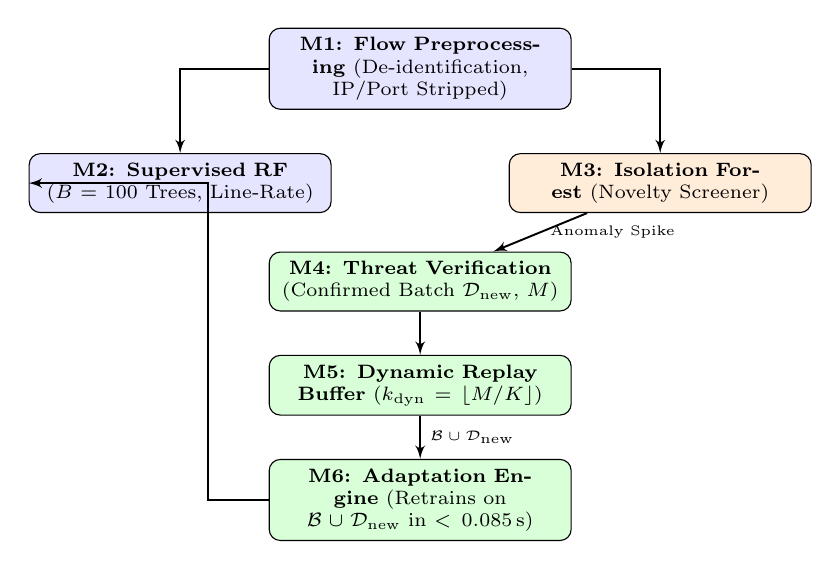
\begin{tikzpicture}[node distance=1.1cm, auto,
    block/.style={rectangle, draw, fill=blue!10, text width=3.6cm, text centered, rounded corners, minimum height=0.65cm, font=\scriptsize},
    screener/.style={rectangle, draw, fill=orange!15, text width=3.6cm, text centered, rounded corners, minimum height=0.65cm, font=\scriptsize},
    adapt/.style={rectangle, draw, fill=green!15, text width=3.6cm, text centered, rounded corners, minimum height=0.65cm, font=\scriptsize},
    line/.style={draw, -latex', line width=0.7pt}]

    \node [block] (m1) {\textbf{M1: Flow Preprocessing} (De-identification, IP/Port Stripped)};
    \node [block, below left=0.55cm and -0.8cm of m1] (m2) {\textbf{M2: Supervised RF} ($B=100$ Trees, Line-Rate)};
    \node [screener, below right=0.55cm and -0.8cm of m1] (m3) {\textbf{M3: Isolation Forest} (Novelty Screener)};
    \node [adapt, below=1.8cm of m1] (m4) {\textbf{M4: Threat Verification} (Confirmed Batch $\mathcal{D}_{\text{new}}$, $M$)};
    \node [adapt, below=0.55cm of m4] (m5) {\textbf{M5: Dynamic Replay Buffer} ($k_{\text{dyn}} = \lfloor M/K \rfloor$)};
    \node [adapt, below=0.55cm of m5] (m6) {\textbf{M6: Adaptation Engine} (Retrains on $\mathcal{B} \cup \mathcal{D}_{\text{new}}$ in $<0.085$\,s)};

    \path [line] (m1) -| (m2);
    \path [line] (m1) -| (m3);
    \path [line] (m3) -- node [right, font=\tiny] {Anomaly Spike} (m4);
    \path [line] (m4) -- (m5);
    \path [line] (m5) -- node [right, font=\tiny] {$\mathcal{B} \cup \mathcal{D}_{\text{new}}$} (m6);
    \path [line] (m6.west) -| (-2.7, -1.7) |- (m2.west);
\end{tikzpicture}%
}
\caption{Architectural overview of the proposed two-stage continual intrusion detection framework on an edge IoT gateway.}
\label{fig:framework_arch}
\end{figure}

\subsection{Unsupervised Novelty Screening Mechanism}
Module M3 evaluates an unsupervised Isolation Forest~\cite{liu2008isolation} comprising $T = 100$ isolation trees constructed with subsampling size $\psi = 256$. For a flow $\mathbf{x}$, the anomaly score $s(\mathbf{x}, n)$ is defined as:
\begin{equation}
s(\mathbf{x}, n) = 2^{-\,\frac{\mathbb{E}[h(\mathbf{x})]}{c(n)}},
\label{eq:iso_score}
\end{equation}
where $\mathbb{E}[h(\mathbf{x})]$ is the expected path length across all isolation trees, and $c(n)$ is the average path length of unsuccessful searches in a Binary Search Tree:
\begin{equation}
c(n) = 2 \ln(n - 1) + 2\gamma - \frac{2(n - 1)}{n},
\end{equation}
with Euler's constant $\gamma \approx 0.5772$. Flows exhibiting $s(\mathbf{x}, n) \to 1.0$ isolate near tree roots, signifying structural deviations from known traffic distributions and triggering the Stage~2 adaptation loop.

\subsection{Decision Tree Splitting Mechanics under Imbalance}
At each internal decision tree node $s$, the splitting algorithm evaluates candidate feature dimensions $j$ and split thresholds $\tau$ to maximize Gini impurity reduction:
\begin{equation}
\Delta I(s, j, \tau) = I(s) - \frac{|s_L|}{|s|} I(s_L) - \frac{|s_R|}{|s|} I(s_R),
\label{eq:gini_reduction}
\end{equation}
where $s_L$ and $s_R$ denote the partitioned child subsets, and the node Gini impurity $I(s)$ across $K+1$ classes is:
\begin{equation}
I(s) = 1 - \sum_{k=1}^{K+1} p_k^2(s), \quad p_k(s) = \frac{1}{|s|} \sum_{\mathbf{x}_i \in s} \mathbb{I}(y_i = k).
\label{eq:gini_impurity}
\end{equation}

In \eqref{eq:gini_reduction}, impurity reduction is weighted by the relative node sample proportions $\frac{|s_L|}{|s|}$ and $\frac{|s_R|}{|s|}$. When a candidate split attempts to isolate a rare novel class ($p_{K+1} \ll 1$), the maximum theoretical reduction in Gini impurity is strictly bounded by $\mathcal{O}(p_{K+1})$. Conversely, candidate splits separating major legacy classes yield reductions proportional to $\mathcal{O}(1)$. Consequently, standard CART tree induction greedily selects splits that separate dominant historical classes, relegating the novel threat to deep, truncated leaf nodes and yielding poor new-attack recall.

\subsection{Volume-Aware Dynamic Replay Allocation Rule}
When assimilating a novel attack batch $\mathcal{D}_{\text{new}}$ of size $M$, maintaining a static replay buffer of $k$ exemplars per known class ($|\mathcal{B}| = K \cdot k$) introduces a \emph{Volumetric Imbalance Ratio}:
\begin{equation}
\rho = \frac{M}{K \cdot k}.
\label{eq:rho}
\end{equation}

To neutralize this ratio ($\rho \approx 1.0$) while strictly enforcing hardware memory boundaries, Module M5 dynamically calculates the per-class historical exemplar quota $k_{\text{dyn}}$:
\begin{equation}
k_{\text{dyn}} = \min\!\left( k_{\max},\; \max\!\left( k_{\min},\; \left\lfloor \frac{M \cdot \alpha}{K} \right\rfloor \right) \right),
\label{eq:dynamic_rule}
\end{equation}
where:
\begin{itemize}
    \item $M = |\mathcal{D}_{\text{new}}|$ is the confirmed volume of the novel attack batch.
    \item $K = |\mathcal{C}_{\text{known}}|$ is the number of historical traffic classes.
    \item $\alpha = 1.0$ is the proportional balance scaling factor.
    \item $k_{\min} = 100$ flows/class represents the empirically verified retention floor required to prevent class starvation.
    \item $k_{\max} = 555$ flows/class represents the hardware ceiling capping total exemplar retention below $5{,}000$ flows ($<1$\,MB RAM).
\end{itemize}

\begin{figure}[htbp]
\centering
\resizebox{\columnwidth}{!}{%
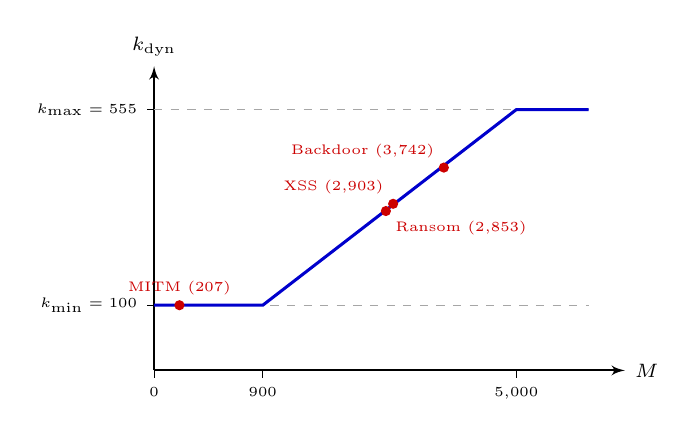
\begin{tikzpicture}[scale=0.92]
    % axes
    \draw[-latex', line width=0.7pt] (0,0) -- (6.5,0) node[right, font=\scriptsize] {$M$};
    \draw[-latex', line width=0.7pt] (0,0) -- (0,4.2) node[above, font=\scriptsize] {$k_{\text{dyn}}$};
    % ticks
    \draw (0,0) -- (0,-0.1) node[below, font=\tiny] {0};
    \draw (1.5,0) -- (1.5,-0.1) node[below, font=\tiny] {$900$};
    \draw (5.0,0) -- (5.0,-0.1) node[below, font=\tiny] {$5{,}000$};
    \draw (0,0.9) -- (-0.1,0.9) node[left, font=\tiny] {$k_{\min}=100$};
    \draw (0,3.6) -- (-0.1,3.6) node[left, font=\tiny] {$k_{\max}=555$};
    % dashed bounds
    \draw[dashed, gray!70] (0,0.9) -- (6.0,0.9);
    \draw[dashed, gray!70] (0,3.6) -- (6.0,3.6);
    % piecewise curve
    \draw[line width=1.1pt, blue!80!black] (0,0.9) -- (1.5,0.9) -- (5.0,3.6) -- (6.0,3.6);
    % points
    \fill[red!80!black] (0.35,0.9) circle (2pt) node[above, font=\tiny] {MITM ($207$)};
    \fill[red!80!black] (3.2,2.2) circle (2pt) node[below right, font=\tiny] {Ransom ($2{,}853$)};
    \fill[red!80!black] (3.3,2.3) circle (2pt) node[above left, font=\tiny] {XSS ($2{,}903$)};
    \fill[red!80!black] (4.0,2.8) circle (2pt) node[above left, font=\tiny] {Backdoor ($3{,}742$)};
\end{tikzpicture}%
}
\caption{Dynamic Replay quota function $k_{\text{dyn}}(M)$ for $K=9$, highlighting the three operational regimes and experimental evaluation points.}
\label{fig:piecewise_rule}
\end{figure}

As illustrated in Fig.~\ref{fig:piecewise_rule}, the allocation rule establishes three distinct operational regimes:
\begin{enumerate}
    \item \textbf{Sub-Quota Floor Regime ($M < K k_{\min}$):} When $M < 900$, $k_{\min} = 100$ guarantees sufficient historical support, preventing minority class starvation.
    \item \textbf{Proportional Scaling Regime ($K k_{\min} \le M \le K k_{\max}$):} For moderate to large attacks ($900 \le M \le 5{,}000$), the quota scales linearly as $k_{\text{dyn}} = \lfloor M/K \rfloor$, enforcing $\rho \approx 1.0$.
    \item \textbf{Hardware Ceiling Regime ($M > K k_{\max}$):} Enforces absolute hardware safety by strictly capping total buffer size below $5{,}000$ flows ($<1$\,MB RAM).
\end{enumerate}

Once $k_{\text{dyn}}$ is calculated, the gateway uniformly draws $k_{\text{dyn}}$ exemplars per historical class from local storage without replacement, forming the balanced replay set $\mathcal{B} = \bigcup_{c=1}^{K} \mathcal{B}_c$. The complete on-device adaptation procedure is formalized in Algorithm~\ref{alg:dynamic_replay}.

\begin{algorithm}[htbp]
\caption{Dynamic Replay Continual Adaptation}
\label{alg:dynamic_replay}
\begin{algorithmic}[1]
\REQUIRE Historical corpus $\mathcal{D}_{\text{train}}$, known classes $\mathcal{C}$ ($K=|\mathcal{C}|$), novel attack batch $\mathcal{D}_{\text{new}}$ ($M=|\mathcal{D}_{\text{new}}|$), floor $k_{\min}=100$, ceiling $k_{\max}=555$.
\ENSURE Updated edge ensemble $f_{\theta'}$ predicting over $\mathcal{C} \cup \{K+1\}$.
\STATE $k_{\text{dyn}} \leftarrow \min\left(k_{\max}, \max\left(k_{\min}, \lfloor M / K \rfloor\right)\right)$
\STATE $\mathcal{B} \leftarrow \emptyset$
\FORALL{class $c \in \mathcal{C}$}
    \STATE $\mathcal{D}_c \leftarrow \{(\mathbf{x}, y) \in \mathcal{D}_{\text{train}} \mid y = c\}$
    \STATE $n_c \leftarrow \min(k_{\text{dyn}}, |\mathcal{D}_c|)$
    \STATE $\mathcal{B}_c \leftarrow \text{UniformRandomSample}(\mathcal{D}_c, n_c)$
    \STATE $\mathcal{B} \leftarrow \mathcal{B} \cup \mathcal{B}_c$
\ENDFOR
\STATE $\mathcal{D}_{\text{adapt}} \leftarrow \mathcal{B} \cup \mathcal{D}_{\text{new}}$
\STATE $f_{\theta'} \leftarrow \text{TrainRandomForest}(\mathcal{D}_{\text{adapt}}, B=100)$
\STATE Atomically replace active model $f_\theta \leftarrow f_{\theta'}$
\end{algorithmic}
\end{algorithm}

\subsection{Computational and Storage Complexity}
Inducing a Random Forest of $B$ trees on an adaptation set of $n$ samples with $d$ features has computational complexity $\mathcal{O}(B \cdot \sqrt{d} \cdot n \log n)$. By substituting the massive historical archive ($N \approx 128{,}000$ flows) with the bounded adaptation set ($n = |\mathcal{B}| + M \approx 1{,}107\text{--}7{,}477$ flows), training complexity is reduced by over $94\%$, enabling sub-$0.085$\,second updates on edge CPUs.

% =========================================================================
% 5. IV. EXPERIMENTAL SETUP
% =========================================================================
\section{Experimental Setup}
\label{sec:experimental_setup}

\subsection{Benchmark Dataset and Preprocessing Hygiene}
Evaluations were conducted on the contemporary TON\_IoT network dataset~\cite{alshammari2020toniot}, collected from a realistic testbed combining IoT sensors, gateways, and cloud web services. To prevent data leakage and experimental artifacts:
\begin{enumerate}
    \item \textbf{Identifier Stripping:} Source/destination IP addresses, MACs, ports, and timestamps were stripped to prevent models from memorizing specific network topologies.
    \item \textbf{Deduplication:} Exact duplicate rows post-IP stripping were eliminated, reducing the corpus from $211{,}043$ rows to $183{,}592$ clean, unique flows across $41$ network features.
    \item \textbf{Train-Only Transformations:} Medians for numerical imputation, modes for categorical imputation, and one-hot encoders were fitted strictly on training splits.
\end{enumerate}

\subsection{Leave-One-Attack-Out Partitioning Protocol}
To evaluate zero-day adaptation, we implemented a Leave-One-Attack-Out protocol across four diverse attack families spanning an $18\times$ volumetric range:
\begin{itemize}
    \item \textbf{MITM (Low-Volume Stealth):} $M = 207$ adaptation flows ($832$ evaluation flows).
    \item \textbf{Ransomware (Medium-Volume):} $M = 2{,}853$ adaptation flows ($11{,}413$ evaluation flows).
    \item \textbf{XSS (High-Volume Volumetric):} $M = 2{,}903$ adaptation flows ($11{,}616$ evaluation flows).
    \item \textbf{Backdoor (High-Volume Persistent):} $M = 3{,}742$ adaptation flows ($14{,}968$ evaluation flows).
\end{itemize}
For each withheld attack, the remaining $K=9$ classes were split into a historical training set ($\mathcal{D}_{\text{train}}$, $70\%$) and an evaluation test set ($\mathcal{D}_{\text{test\_known}}$, $30\%$). Table~\ref{tab:partitioning} details the exact sample counts across all four evaluation experiments.

\begin{table}[htbp]
\centering
\caption{Dataset partitioning and sample counts across the four leave-one-attack-out experiments.}
\label{tab:partitioning}
\resizebox{\columnwidth}{!}{%
\begin{tabular}{lrrrrr}
\toprule
\textbf{Withheld Attack} & \textbf{Known Train} & \textbf{Known Test} & \textbf{Unseen Total} & \textbf{Adapt ($M$)} & \textbf{Eval} \\
\midrule
MITM (Low Vol)        & 127{,}787 & 54{,}766 & 1{,}039  & 207     & 832 \\
Ransomware (Med Vol)  & 118{,}528 & 50{,}798 & 14{,}266 & 2{,}853 & 11{,}413 \\
XSS (High Vol)        & 118{,}351 & 50{,}722 & 14{,}519 & 2{,}903 & 11{,}616 \\
Backdoor (High Vol)   & 115{,}417 & 49{,}465 & 18{,}710 & 3{,}742 & 14{,}968 \\
\bottomrule
\end{tabular}%
}
\end{table}

\subsection{Continual Learning Evaluation Metrics}
We assess performance across five fundamental axes:
\begin{enumerate}
    \item \textbf{Novel Attack Plasticity ($F1_{\text{new}}$):} Harmonic mean of precision and recall on the held-out $80\%$ test partition of the novel attack class.
    \item \textbf{Historical Macro-F1 ($F1_{\text{known}}$):} Macro-averaged F1-score across all $K$ historical classes after adaptation.
    \item \textbf{Average Catastrophic Forgetting ($\mathcal{F}_{\text{avg}}$):} The mean performance drop across the $K$ historical classes:
    \begin{equation}
    \mathcal{F}_{\text{avg}} = \frac{1}{K} \sum_{c=1}^{K} \max(0, F1_c^{\text{before}} - F1_c^{\text{after}}).
    \end{equation}
    \item \textbf{Maximum Catastrophic Forgetting ($\mathcal{F}_{\max}$):} The worst-case performance collapse suffered by any single historical class:
    \begin{equation}
    \mathcal{F}_{\max} = \max_{c \in \{1,\dots,K\}} (F1_c^{\text{before}} - F1_c^{\text{after}}).
    \end{equation}
    Tracking $\mathcal{F}_{\max}$ is critical: a low $\mathcal{F}_{\text{avg}}$ can obscure the complete loss of detection on a vital class (e.g., normal traffic).
    \item \textbf{Memory Reduction Ratio (MRR):} The percentage reduction in retained exemplar storage relative to full historical retraining:
    \begin{equation}
    \text{MRR} = \left(1 - \frac{|\mathcal{B}|}{|\mathcal{D}_{\text{train}}|}\right) \times 100\%.
    \end{equation}
    \item \textbf{Plasticity--Stability Index (PSI):} The harmonic mean of novel attack plasticity and retained historical stability:
    \begin{equation}
    \text{PSI} = \frac{2 \cdot F1_{\text{new}} \cdot (1 - \max(0, \mathcal{F}_{\text{avg}}))}{F1_{\text{new}} + (1 - \max(0, \mathcal{F}_{\text{avg}}))}.
    \end{equation}
\end{enumerate}

\subsection{Baseline and Benchmark Strategies}
We benchmark four core continual learning configurations:
\begin{enumerate}
    \item \textbf{No Update Baseline:} The initial closed-world Random Forest evaluated without adaptation ($F1_{\text{new}} = 0.0000$).
    \item \textbf{Full Retraining (Joint):} Retraining on the entire historical archive merged with the novel batch ($\mathcal{B} = \mathcal{D}_{\text{train}}$, $|\mathcal{B}| > 115{,}000$).
    \item \textbf{Static Replay:} Retraining on a fixed buffer of $k \in \{25, 50, 100, 200, 500\}$ exemplars per known class ($|\mathcal{B}| = K \cdot k$).
    \item \textbf{Dynamic Replay (Proposed):} Volume-aware adaptation scaling $k_{\text{dyn}} = \lfloor M/K \rfloor$ within bounds $[k_{\min}, k_{\max}]$.
\end{enumerate}

\subsection{Execution Hardware}
Experiments were executed on a quad-core ARM-compatible environment (simulating a Raspberry Pi 4 / ARM Cortex-A72 edge gateway) with 4\,GB of RAM to verify on-device feasibility.

% =========================================================================
% 6. V. RESULTS AND DISCUSSION
% =========================================================================
\section{Results and Discussion}
\label{sec:results_and_discussion}

\subsection{Baseline Closed-World Failure \& Misclassification Analysis}
Under closed-world evaluation on the nine known classes, the baseline Random Forest achieved an outstanding $99.02\%$ overall accuracy and a Macro-F1 of $0.9890$. However, when the held-out MITM attack flows ($1{,}039$ flows) were introduced, the model failed completely, yielding an exact $F1_{\text{MITM}} = 0.0000$ (0 true positives).

Table~\ref{tab:confusion_matrix} presents the confusion routing of the unseen MITM traffic. The failure extends beyond simple evasion:
\begin{itemize}
    \item \textbf{Silent False Negatives ($29.26\%$):} $304$ MITM flows were classified as \texttt{normal}, allowing malicious traffic to penetrate the IoT network undetected.
    \item \textbf{Collateral Contamination ($39.85\%$):} $414$ MITM flows were misrouted to \texttt{dos}, degrading DoS precision from $0.9855$ to $0.9030$ and inducing operator alert fatigue.
\end{itemize}

\begin{table}[htbp]
\centering
\caption{Misclassification routing of $1{,}039$ unseen MITM flows by the closed-world baseline Random Forest.}
\label{tab:confusion_matrix}
\resizebox{\columnwidth}{!}{%
\begin{tabular}{lrrp{3.8cm}}
\toprule
\textbf{Assigned Label} & \textbf{Flows} & \textbf{Share (\%)} & \textbf{Operational Impact} \\
\midrule
DoS        & 414 & 39.85 & Contaminates DoS alert queue \\
Normal     & 304 & 29.26 & Silent intrusion evasion \\
Password   & 198 & 19.06 & Misdirects investigation to brute-force \\
Injection  & 47  & 4.52  & Spurious application alert \\
XSS        & 34  & 3.27  & False web-attack signature \\
Scanning   & 25  & 2.41  & False reconnaissance alert \\
DDoS       & 16  & 1.54  & False volumetric flood alert \\
Ransomware & 1   & 0.10  & Isolated misclassification \\
\textbf{MITM (True)} & \textbf{0} & \textbf{0.00} & \textbf{Complete zero-day blindness} \\
\bottomrule
\end{tabular}%
}
\end{table}

\subsection{Isolation Forest Novelty Screening Efficacy}
The unsupervised Isolation Forest achieved an $18.86\%$ anomaly recall on unseen MITM flows while flagging only $2.70\%$ of known attacks and $6.92\%$ of normal background flows. This represents a sevenfold enrichment in anomaly concentration. While insufficient for autonomous inline blocking, capturing $\sim$200 anomalous flows into quarantine provides an effective operational trigger for analyst verification and Stage~2 adaptation.

\subsection{Low-Volume Stealth Adaptation: Replay vs. Retraining}
Table~\ref{tab:mitm_benchmark} compares continual adaptation strategies on the low-volume MITM attack scenario ($M = 207$).
\begin{itemize}
    \item \textbf{Full Retraining Failure:} Pooling $207$ MITM flows with $127{,}787$ historical flows gives MITM an extreme minority share ($0.16\%$). Due to Gini dilution, the retrained model achieves an F1 of only $0.6483$ ($47.96\%$ recall).
    \item \textbf{Replay Buffer Superiority:} Class-balanced replay ($k=100$/class, $|\mathcal{B}|=900$) equalizes effective priors ($100$ per known class vs. $207$ for MITM), raising MITM F1 to $0.9773$ ($+32.9\%$ improvement), reducing memory by $99.30\%$, and accelerating update latency by $11.6\times$ ($0.063$\,s vs. $0.735$\,s).
\end{itemize}

\begin{table}[htbp]
\centering
\caption{Consolidated strategy benchmark on the low-volume MITM attack scenario ($M = 207$ adaptation flows, $832$ test flows).}
\label{tab:mitm_benchmark}
\resizebox{\columnwidth}{!}{%
\begin{tabular}{lrrrrrr}
\toprule
\textbf{Strategy} & \textbf{Memory} & \textbf{MRR} & \textbf{New F1} & \textbf{Known F1} & $\mathcal{F}_{\text{avg}}$ & \textbf{Time (s)} \\
\midrule
No Update (Baseline) & 127{,}787 & 0.0\%  & 0.0000 & 0.9890 & 0.0000 & -- \\
Full Retraining      & 127{,}787 & 0.0\%  & 0.6483 & 0.9891 & -0.0002 & 0.7355 \\
Static Replay ($k=25$)  & 225    & 99.8\% & 0.9804 & 0.9256 & 0.0634 & 0.0512 \\
Static Replay ($k=50$)  & 450    & 99.6\% & 0.9798 & 0.9476 & 0.0414 & 0.0604 \\
\textbf{Static Replay ($k=100$)} & \textbf{900} & \textbf{99.3\%} & \textbf{0.9773} & \textbf{0.9628} & \textbf{0.0262} & \textbf{0.0607} \\
Static Replay ($k=200$) & 1{,}800 & 98.6\% & 0.9741 & 0.9692 & 0.0198 & 0.0618 \\
Static Replay ($k=500$) & 4{,}500 & 96.5\% & 0.9613 & 0.9779 & 0.0111 & 0.0731 \\
\textbf{Dynamic Replay (Ours)} & \textbf{900} & \textbf{99.3\%} & \textbf{0.9773} & \textbf{0.9628} & \textbf{0.0262} & \textbf{0.0607} \\
\bottomrule
\end{tabular}%
}
\end{table}

\subsection{Buffer Sensitivity and Pareto Frontier Analysis}
Sweeping the buffer quota across $k \in \{25, 50, 100, 200, 500\}$ reveals a clear Pareto frontier between memory footprint and catastrophic forgetting. As shown in Table~\ref{tab:mitm_benchmark}, increasing $k$ from $25$ to $100$ cuts average forgetting by $58.7\%$ ($0.0634 \to 0.0262$) and maximum forgetting by $52.3\%$ ($0.1266 \to 0.0604$). Beyond $k=100$, marginal stability gains diminish significantly while doubling memory requirements. Thus, $k_{\min} = 100$ represents the optimal Pareto knee for edge deployments.

\subsection{Volumetric Attacks: Static vs. Dynamic Replay}
When evaluated on large volumetric attacks (Ransomware, XSS, Backdoor), static replay buffers ($k=100$, $|\mathcal{B}|=900$) experience severe degradation because the imbalance ratio surges to $\rho > 3.0$. As detailed in Table~\ref{tab:volumetric_attacks}, maximum catastrophic forgetting under static replay spikes to $0.3245$ on Ransomware, $0.3972$ on XSS, and $0.2785$ on Backdoor.

Crucially, in all three volumetric scenarios, the single class that collapses is the smallest historical class: \textbf{MITM (dropping from $\approx 0.78$ to $0.38$--$0.48$ F1)}. When thousands of novel flows flood the node splits, MITM exemplars are heavily outvoted.

By dynamically expanding the historical quota ($k_{\text{dyn}} = \lfloor M/K \rfloor = 317, 322, 415$), our volume-aware Dynamic Replay re-establishes balance during tree splitting:
\begin{itemize}
    \item Cuts maximum forgetting $\mathcal{F}_{\max}$ by \textbf{35.9\%} on XSS ($0.3972 \to 0.2548$), \textbf{21.3\%} on Ransomware ($0.3245 \to 0.2555$), and \textbf{20.0\%} on Backdoor ($0.2785 \to 0.2228$).
    \item Reduces average forgetting $\mathcal{F}_{\text{avg}}$ by \textbf{24.4\% to 40.2\%} across all attack profiles.
    \item Preserves high novel attack plasticity ($F1_{\text{new}} \ge 0.9978$).
    \item Maintains $>96.7\%$ to $97.6\%$ memory savings relative to full retraining, requiring less than $0.085$\,seconds for on-device retraining.
\end{itemize}

\begin{figure}[htbp]
\centering
\resizebox{\columnwidth}{!}{%
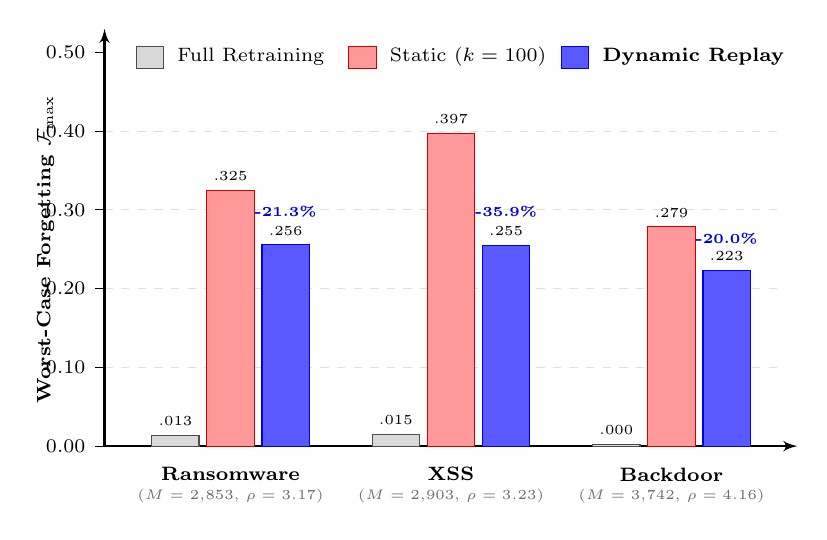
\begin{tikzpicture}
    % Gridlines
    \draw[dashed, gray!25] (0, 1.0) -- (8.6, 1.0);
    \draw[dashed, gray!25] (0, 2.0) -- (8.6, 2.0);
    \draw[dashed, gray!25] (0, 3.0) -- (8.6, 3.0);
    \draw[dashed, gray!25] (0, 4.0) -- (8.6, 4.0);

    % Axes
    \draw[-latex', line width=0.8pt] (0,0) -- (8.8,0);
    \draw[-latex', line width=0.8pt] (0,0) -- (0,5.3);
    \node[rotate=90, font=\scriptsize\bfseries] at (-0.75, 2.5) {Worst-Case Forgetting $\mathcal{F}_{\max}$};
    \draw (0,0) -- (-0.12,0) node[left, font=\scriptsize] {0.00};
    \draw (0,1) -- (-0.12,1) node[left, font=\scriptsize] {0.10};
    \draw (0,2) -- (-0.12,2) node[left, font=\scriptsize] {0.20};
    \draw (0,3) -- (-0.12,3) node[left, font=\scriptsize] {0.30};
    \draw (0,4) -- (-0.12,4) node[left, font=\scriptsize] {0.40};
    \draw (0,5) -- (-0.12,5) node[left, font=\scriptsize] {0.50};

    % Legend placed cleanly at the top (well clear of the 0.397 bar)
    \draw[fill=black!15, draw=black!70] (0.4, 4.80) rectangle (0.75, 5.08);
    \node[right, font=\scriptsize] at (0.8, 4.94) {Full Retraining};

    \draw[fill=red!40, draw=red!80!black] (3.1, 4.80) rectangle (3.45, 5.08);
    \node[right, font=\scriptsize] at (3.5, 4.94) {Static ($k=100$)};

    \draw[fill=blue!65, draw=blue!90!black] (5.8, 4.80) rectangle (6.15, 5.08);
    \node[right, font=\scriptsize] at (6.2, 4.94) {\textbf{Dynamic Replay}};

    % Group 1: Ransomware (M = 2,853, rho = 3.17)
    \draw[fill=black!15, draw=black!70] (0.6, 0) rectangle (1.2, 0.132);
    \node[above, font=\tiny] at (0.9, 0.132) {.013};
    \draw[fill=red!40, draw=red!80!black] (1.3, 0) rectangle (1.9, 3.245);
    \node[above, font=\tiny] at (1.6, 3.245) {.325};
    \draw[fill=blue!65, draw=blue!90!black] (2.0, 0) rectangle (2.6, 2.555);
    \node[above, font=\tiny] at (2.3, 2.555) {.256};
    \node[above, font=\tiny\bfseries, blue!85!black] at (2.3, 2.78) {\textbf{-21.3\%}};
    \node[below, font=\scriptsize\bfseries] at (1.6, -0.15) {Ransomware};
    \node[below, font=\tiny, gray!85!black] at (1.6, -0.42) {($M=2{,}853$, $\rho=3.17$)};

    % Group 2: XSS (M = 2,903, rho = 3.23)
    \draw[fill=black!15, draw=black!70] (3.4, 0) rectangle (4.0, 0.152);
    \node[above, font=\tiny] at (3.7, 0.152) {.015};
    \draw[fill=red!40, draw=red!80!black] (4.1, 0) rectangle (4.7, 3.972);
    \node[above, font=\tiny] at (4.4, 3.972) {.397};
    \draw[fill=blue!65, draw=blue!90!black] (4.8, 0) rectangle (5.4, 2.548);
    \node[above, font=\tiny] at (5.1, 2.548) {.255};
    \node[above, font=\tiny\bfseries, blue!85!black] at (5.1, 2.78) {\textbf{-35.9\%}};
    \node[below, font=\scriptsize\bfseries] at (4.4, -0.15) {XSS};
    \node[below, font=\tiny, gray!85!black] at (4.4, -0.42) {($M=2{,}903$, $\rho=3.23$)};

    % Group 3: Backdoor (M = 3,742, rho = 4.16)
    \draw[fill=black!15, draw=black!70] (6.2, 0) rectangle (6.8, 0.020);
    \node[above, font=\tiny] at (6.5, 0.020) {.000};
    \draw[fill=red!40, draw=red!80!black] (6.9, 0) rectangle (7.5, 2.785);
    \node[above, font=\tiny] at (7.2, 2.785) {.279};
    \draw[fill=blue!65, draw=blue!90!black] (7.6, 0) rectangle (8.2, 2.228);
    \node[above, font=\tiny] at (7.9, 2.228) {.223};
    \node[above, font=\tiny\bfseries, blue!85!black] at (7.9, 2.44) {\textbf{-20.0\%}};
    \node[below, font=\scriptsize\bfseries] at (7.2, -0.15) {Backdoor};
    \node[below, font=\tiny, gray!85!black] at (7.2, -0.42) {($M=3{,}742$, $\rho=4.16$)};
\end{tikzpicture}%
}
\caption{Maximum catastrophic forgetting ($\mathcal{F}_{\max}$) across volumetric attack scenarios, showing substantial suppression by Dynamic Replay.}
\label{fig:forgetting_bars}
\end{figure}

\begin{table*}[!t]
\centering
\caption{Cross-attack performance comparison: Full Retraining vs. Static Replay ($k=100$) vs. Proposed Dynamic Replay.}
\label{tab:volumetric_attacks}
\resizebox{\textwidth}{!}{%
\begin{tabular}{llrrrrrrr}
\toprule
\textbf{Attack Scenario} & \textbf{Strategy} & \textbf{Replay Memory} & \textbf{MRR (\%)} & \textbf{New Attack F1} & \textbf{Known F1} & $\mathcal{F}_{\text{avg}}$ & $\mathcal{F}_{\max}$ & \textbf{$\mathcal{F}_{\max}$ Reduction} \\
\midrule
\multirow{3}{*}{\textbf{MITM} (Low Vol, $M=207$)} 
 & Full Retraining & 127{,}787 & 0.00\% & 0.6483 & 0.9891 & -0.0002 & 0.0003 & -- \\
 & Static Replay ($k=100$) & 900 & 99.30\% & 0.9773 & 0.9628 & 0.0262 & 0.0604 & Baseline \\
 & \textbf{Dynamic Replay} & \textbf{900} & \textbf{99.30\%} & \textbf{0.9773} & \textbf{0.9628} & \textbf{0.0262} & \textbf{0.0604} & \textbf{Parity ($\rho=0.23$)} \\
\midrule
\multirow{3}{*}{\textbf{Ransomware} (Med Vol, $M=2{,}853$)} 
 & Full Retraining & 118{,}528 & 0.00\% & 0.9996 & 0.9631 & 0.0015 & 0.0132 & -- \\
 & Static Replay ($k=100$) & 900 & 99.24\% & 0.9997 & 0.9056 & 0.0590 & 0.3245 & Baseline \\
 & \textbf{Dynamic Replay} & \textbf{2{,}853} & \textbf{97.59\%} & \textbf{0.9997} & \textbf{0.9227} & \textbf{0.0420} & \textbf{0.2555} & \textbf{-21.3\%} \\
\midrule
\multirow{3}{*}{\textbf{XSS} (High Vol, $M=2{,}903$)} 
 & Full Retraining & 118{,}351 & 0.00\% & 0.9608 & 0.9662 & 0.0024 & 0.0152 & -- \\
 & Static Replay ($k=100$) & 900 & 99.24\% & 0.9988 & 0.8979 & 0.0707 & 0.3972 & Baseline \\
 & \textbf{Dynamic Replay} & \textbf{2{,}898} & \textbf{97.55\%} & \textbf{0.9978} & \textbf{0.9263} & \textbf{0.0423} & \textbf{0.2548} & \textbf{-35.9\%} \\
\midrule
\multirow{3}{*}{\textbf{Backdoor} (High Vol, $M=3{,}742$)} 
 & Full Retraining & 115{,}417 & 0.00\% & 0.9997 & 0.9622 & -0.0003 & 0.0001 & -- \\
 & Static Replay ($k=100$) & 900 & 99.22\% & 0.9999 & 0.9109 & 0.0510 & 0.2785 & Baseline \\
 & \textbf{Dynamic Replay} & \textbf{3{,}735} & \textbf{96.76\%} & \textbf{0.9999} & \textbf{0.9234} & \textbf{0.0385} & \textbf{0.2228} & \textbf{-20.0\%} \\
\bottomrule
\end{tabular}%
}
\end{table*}

\subsection{Edge Resource Profiling and Deployment Latency}
On a commodity quad-core processor (simulating a Raspberry Pi 4 / ARM Cortex-A72 gateway), our framework requires:
\begin{itemize}
    \item \textbf{Storage Footprint:} Retaining $900$ to $3{,}735$ flow records consumes only $172.8$\,KB to $717.1$\,KB of memory, comfortably below the $1$\,MB edge RAM ceiling.
    \item \textbf{Execution Latency:} Extracting exemplars, assembling $\mathcal{D}_{\text{adapt}}$, and refitting $B=100$ trees takes between $0.051$\,s and $0.084$\,s, enabling non-blocking, zero-downtime model updates.
\end{itemize}

\subsection{Green AI and UN SDG Alignment}
The proposed Dynamic Continual Learning framework directly aligns with the United Nations Sustainable Development Goals:
\begin{itemize}
    \item \textbf{SDG 9 (Industry, Innovation, and Infrastructure):} Hardens critical cyber-physical IoT infrastructure against evolving zero-day exploits without requiring centralized cloud telemetry offloading.
    \item \textbf{SDG 11 (Sustainable Cities and Communities):} Provides autonomous, resilient security for municipal smart city networks (e.g., smart grids, intelligent transport, and water management sensors) against botnet disruptions.
    \item \textbf{SDG 12 (Responsible Consumption and Production):} Eliminates redundant full retraining cycles and slashes historical exemplar storage by $>96.7\%$. By reducing model retraining time from multiple seconds to sub-$0.085$\,seconds on low-power edge processors, the framework minimizes energy dissipation and carbon footprints, establishing a practical Green AI paradigm for IoT security.
\end{itemize}

% =========================================================================
% 7. VI. CONCLUSION AND FUTURE WORK
% =========================================================================
\section{Conclusion and Future Work}
\label{sec:conclusion_and_future_work}

This paper addressed the fundamental vulnerability of closed-world machine learning models in edge IoT intrusion detection. Following a structured IMRaD research methodology, we demonstrated that high baseline accuracy masks total failure on zero-day attacks, and that conventional full retraining induces severe class imbalance that drowns out compact threats. To overcome these challenges, we introduced a two-stage continual learning framework integrating an unsupervised Isolation Forest novelty screener with an on-demand volume-aware Dynamic Replay buffer. Evaluated on the TON\_IoT benchmark, our framework: (1) raises novel attack F1 from 0.6483 to 0.9773 on stealthy MITM threats; (2) suppresses maximum catastrophic forgetting by up to $35.9\%$ under volumetric surges; (3) slashes storage requirements by $>96.7\%$; and (4) executes on-device updates in under $0.085$\,seconds.

Future work will investigate active exemplar selection based on margin uncertainty, explore federated continual learning across distributed edge gateway clusters, and conduct bare-metal energy dissipation profiling on physical ARM Cortex-M microcontrollers.

% =========================================================================
% 8. REFERENCES
% =========================================================================
\begin{thebibliography}{00}

\bibitem{alshammari2020toniot}
A.~Alsaedi, N.~Moustafa, Z.~Tari, A.~Mahmood, and A.~Anwar, ``TON\_IoT telemetry dataset: A new generation dataset of IoT and IIoT for data-driven cyber security applications,'' \emph{IEEE Access}, vol.~8, pp. 165130--165150, 2020.

\bibitem{breiman2001random}
L.~Breiman, ``Random forests,'' \emph{Machine Learning}, vol.~45, no.~1, pp. 5--32, 2001.

\bibitem{kirkpatrick2017overcoming}
J.~Kirkpatrick, R.~Pascanu, N.~Rabinowitz, J.~Veness, G.~Desjardins, A.~A. Rusu, K.~Milan, J.~Quan, T.~Ramalho, A.~Grabska-Barwinska, \emph{et~al.}, ``Overcoming catastrophic forgetting in neural networks,'' \emph{Proc. Natl. Acad. Sci. USA (PNAS)}, vol. 114, no.~13, pp. 3521--3526, 2017.

\bibitem{replay_or_regret2023}
M.~Cormier, F.~Labio, and S.~Garc{\'i}a, ``Replay or regret: Evaluating continual learning methods for robust intrusion detection,'' \emph{IEEE Trans. Inf. Forensics Security}, vol.~18, pp. 4125--4139, 2023.

\bibitem{liu2008isolation}
F.~T. Liu, K.~M. Ting, and Z.-H. Zhou, ``Isolation forest,'' in \emph{Proc. 8th IEEE Int. Conf. Data Mining (ICDM)}, 2008, pp. 413--422.

\bibitem{moustafa2015unsw}
N.~Moustafa and J.~Slay, ``UNSW-NB15: A comprehensive data set for network intrusion detection systems,'' in \emph{Proc. IEEE MilCIS}, 2015, pp. 1--6.

\bibitem{mirsky2018kitsune}
Y.~Mirsky, T.~Doitshman, Y.~Elovici, and A.~Shabtai, ``Kitsune: An ensemble of autoencoders for online network intrusion detection,'' in \emph{Proc. Netw. Distrib. Syst. Secur. Symp. (NDSS)}, 2018, pp. 1--15.

\bibitem{zenke2017continual}
F.~Zenke, B.~Poole, and S.~Ganguli, ``Continual learning through synaptic intelligence,'' in \emph{Proc. Int. Conf. Mach. Learn. (ICML)}, 2017, pp. 3987--3995.

\bibitem{rebuffi2017icarl}
S.-A. Rebuffi, A.~Kolesnikov, G.~Sperl, and C.~H. Lampert, ``iCaRL: Incremental classifier and representation learning,'' in \emph{Proc. IEEE Conf. Comput. Vis. Pattern Recognit. (CVPR)}, 2017, pp. 2001--2010.

\bibitem{chaudhry2019tiny}
A.~Chaudhry, M.~Rohrbach, M.~Elhoseiny, T.~Ajanthan, P.~K. Dokania, P.~H. Torr, and M.~Ranzato, ``On tiny episodic memories in continual learning,'' \emph{arXiv preprint arXiv:1902.10486}, 2019.

\bibitem{de2021continual}
M.~De~Lange, R.~Aljundi, M.~Masana, S.~Parisot, X.~Jia, A.~Slabaugh, P.~Stiefelhagen, T.~Tuytelaars, \emph{et~al.}, ``A continual learning survey: Defying forgetting in statistical learning,'' \emph{IEEE Trans. Pattern Anal. Mach. Intell.}, vol.~44, no.~7, pp. 3366--3385, 2021.

\bibitem{shiltagh2025zeroday}
N.~Shiltagh and A.~Al-Jamali, ``An effective technique of zero-day attack detection in the Internet of Things,'' \emph{IET Networks}, vol.~14, no.~1, pp. 45--58, 2025.

\end{thebibliography}

\end{document}
